% !TEX root = ../main.tex
%
\chapter{Robust Data Storage}
\label{sec:data-storage}

%This chapter will be based on IDM paper and related work (R scripts, IDM formatter, etc...)

\section{Background}

The ability to gain insights from any data set is rooted in good organization of that data.
Large data collections quickly become overwhelming, complex, and site-specific without a comprehensive system for tagging and differentiating data.
None of these qualities are good for developing or deploying easily transferable metrics for evaluating and comparing performance at many GSI sites.
Instead, consistent metadata and uniform data format are two powerful tools for ensuring that data remains accessible and globally applicable in the sense that two data points collected at different sites can be easily understood to measure the same parameter.
The ability to streamline the combination of data from many different sites into a single database with consistent data descriptions has the potential to unlock new insights into performance, long-term and average maintenance needs, and lifespan predictions.
The accessibility of consistently described data reduces the time spent deciphering the meaning, source, and integrity of a dataset.

The need for consistent data definition is not new but has greatly expanded with the decreasing barriers to entry that enable far wider application of monitoring equipment and data collection.
Civil infrastructure has historically taken an approach to building that favors careful planning, site analysis, and construction validation.
The ability to conduct long term monitoring at a wide-spread scale has been lacking due to the difficulty of collecting and analyzing the data necessary at said scale (\cite{DelGrosso2019}).
The ongoing data revolution has the potential to change that, with modern database techniques enabling consistency and accessibility (\cite{Maidment2008,Abdallah2019}).
Several examples of centralized water data repositories exist already including the International Best Management Practices (BMP) database, which provides many observational data points across a range of GSI types and locations (\cite{LIDCenter2004}), the EPA's Storage and Retrieval System (STORET), and USGS' Nation Weather Information System (NWIS).
However, the data in the International BMP Database is largely focused on discrete samples, and the structure of all these systems is not sufficiently standardized to allow for efficient organization of continuously recorded time series data or collaboration with data across different systems.
While discrete data is an important tool in the study of GSI, continuous data is also highly useful and presents a much larger challenge due to the vastly larger scale of the data collected (\cite{Wadzuk2021a}).
A collection of discrete data points may number in the several hundred or perhaps several thousand, while continuous data easily scales to several million values per site over the course of a multi-year study.
A system of standardized "controlled vocabulary" could help alleviate some of these issues (\cite{Maidment2008}), but would require a great effort to sort through many years of historical data, not all of which may be easily identified and traced back to its proper origin.
Therefore, a modern system with the flexibility to accommodate the scope and size of data collected is necessary to enable multi-year, multi-GSI system studies that can fully take advantage of the expansion in data collection (\cite{Wadzuk2021,Meng2017}).

The Consortium of Universities for the Advancement of Hydrologic Studies, Inc (CUAHSI) have created the Observations Data Model (ODM), which aligns better with the needs of continuous monitoring data and has features for publishing data across different research groups (\cite{Horsburgh2008a,Maidment2008}).
However, there are limitations on data categorization because variable and site codes are used to uniquely identify a data point, so sites with multiple identical variables (e.g., two inflow measurements at different locations within a site) are not possible without creating redundant variables.
Additionally, there are data privacy concerns for research sponsors interested in organizing their data without making it publicly available, as required by the included WaterML integrations.
The schema for the ODM provides a robust means for storing time series data, and is flexible enough to be expanded with the additional metadata collected at various VCRWS project sites, including at SMP A on the PennDOT project.
The ODM is the basis for the expanded platform implemented to handle GSI data at VCRWS.

\section{VCRWS Stormwater Infrastructure Data Model (SIDM)}

Recently implemented at VCRWS, the Stormwater Infrastructure Data Model (SIDM), is a modern database approach to disparate data organization using relational tables.
By abstracting the metadata layer of information away, spatial and temporal linkages between data can be stored without repetition of the metadata itself, making storing and accessing data easier and faster.
The SIDM is based on the schema of the ODM and shares many of the same features, but goes a step further by introducing the ability to associate data with specific sample locations within a given site as well as the implementation of protected sharing features.
The web interface was also refreshed to have a modern look and easy navigation.
User permissions and data sharing abilities are facilitated by pages accessible to site administrators.
New metadata definitions for sites, sampling locations, variables, and methods must be created via their respective pages before data related to the new definitions can be imported.
Data import is available to coordinators for each site, allowing the addition of a single data point for discretely sampled data, or uploading a formatted data file for continuous data.

Throughout the development process, the database was designed to align with principles of FAIR (Findable, Accessible, Interoperable, Reusable) data (\cite{Wilkinson2016}). 
The SIDM's updated data format is intended to meet these criteria to enable more robust and sustainable study of data stored within.
The SIDM makes finding data easy through a simple GUI search page with filters for each type of metadata.
The simple, yet effective interface for building queries to search the database allows authorized users the ability to download all data values and associated metadata to a CSV file with the click of a button, making all data easily accessible.
Metadata is stored in data logs, which remain accessible even when their associated data points have been removed.
This has the potential for further analysis with expanded capabilities such as an application programming interface (API) for easy pre-processing and cleaning.
The data model is reusable, as any given combination of space (site, sample location), time, and variable codes uniquely identifies a data point and can be used as a reference for further analysis.
This traceable metadata associated with every data value allows future users to understand what conditions under which the data was collected.
In addition to making data easier to query, this means that auditing work to determine when and how measurement procedures or methods change becomes possible because each new iteration of a data collection method can be tagged with unique metadata.

\subsection{Metadata Standardization and Data Formatting}

The central feature of the SIDM is the relational nature of the metadata abstraction (\cite{Horsburgh2008a}).
Keeping data and metadata separate allows for more efficient storage because there is no duplication of information and for the flexibility to expand the scope of data stored without updating the storage structure.
Each database table uses a primary key column to uniquely identify records.
These primary keys, when used in other related tables to identify pieces of related information, are called foreign keys.
Foreign keys establish the relationship between a data record and its corresponding site, sample location, variable, and other metadata of interest.
Each of these pieces of metadata are stored in their own tables with consistent information describing each record within (Figure \ref{fig:idm-schema}, enlarged in Appendix A).
By linking the related records with the appropriate keys using a unique identifier, duplicate information is not created.
The structure of these relationships allows infinite combinations of spatial and temporal data, while remaining flexible enough to accommodate new or changed data streams without the need for actual structural updates to the data format.

\begin{figure}[ht]
	\centering
	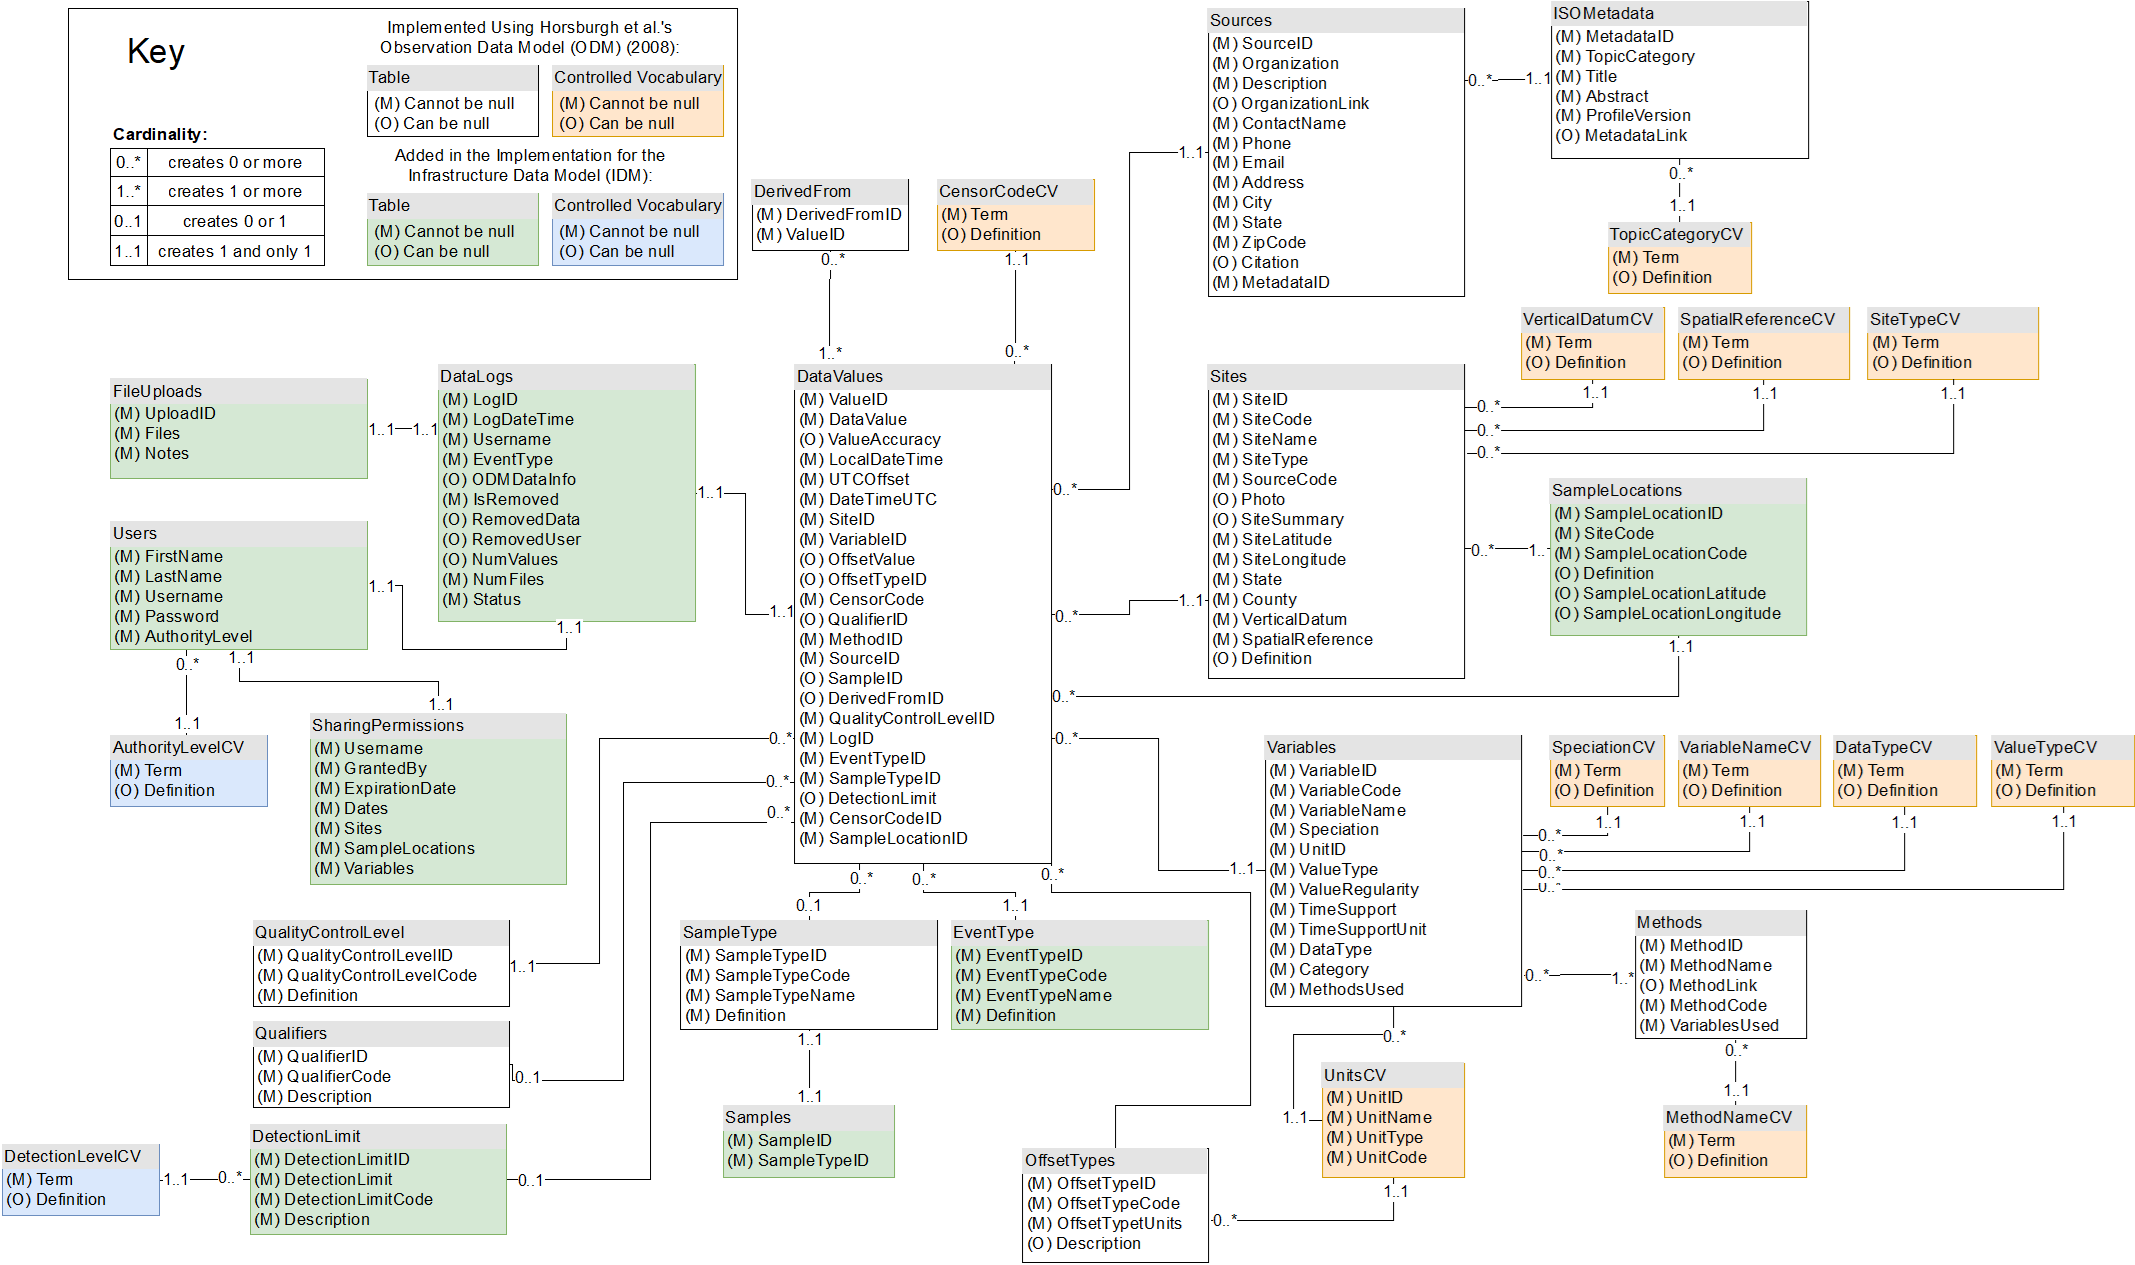
\includegraphics[width=\textwidth]{gfx/chapter-storage/idm_schema.png}
	\caption[SIDM database schema.]{SIDM database schema (Smith et al., submitted).}
	\label{fig:idm-schema}
\end{figure}

Data is collected in a wide format, where each unique variable is stored in its own column and a new row of data is appended to the table for each observational timestamp.
From a storage space perspective, this means that there are $N*M$ rows in the table, where N is the number of observations and M is the number of unique variables.
This is sufficient for storing a dataset related to one and only one site where variables directly correspond to sampling locations.
However, each newly collected variable requires the addition of another column to the table or the creation of a new table, which results in the storage of many missing variables or disjointed data records, respectively.
This approach does not work well when used to combine data from multiple sites, as the column names are the sole form of metadata available to describe variable origins.

An alternative approach, and the one taken by the SIDM, is to abstract the information about a data point's origin (site, sampling location, variable, detection limit, collection method, sample type, and offset information) to separate tables, since this information pertains to many data records.
Storing the identifying metadata only once and referring to it via foreign key constraints in the data records table creates consistency in both metadata format and data record format, which enables faster querying of the data records through the use of covering indices.
Columns in a database containing keys are indexed for faster performance, which requires additional storage space but significantly reduces computational time (\cite{lightstone2010physical}).
A covering index is a composite index made up of a set of all possible columns that could appear in a query, meaning the database only has to consult the index values in order to return results.
This format is referred to as long format, as the number of columns in the data records table is fixed according to the desired metadata for each point and a nearly infinite number of observation rows can be appended without any change to the database schema.
This format only requires that the additional metadata for new variables, sites, or sampling locations be added to the appropriate tables before new data records can be imported.

Transforming continuous monitoring data from wide to long format requires a process called melting, which can be accomplished via packages in nearly any modern general purpose programing language.
During melting, original column names are mapped via a secondary input file containing key-value pairs of corresponding original variable names and the expanded metadata for site code, sample location, and variable name.
This expanded metadata is appended to each data record and then inserted into its own row in the output file, along with the other global inputs available (detection limit, sample type, offset type, event type) since these values are expected to be constant for chunks of continuous monitoring data collected in a single file.
For simplicity of use for those not familiar with programming, a graphical user interface version of this process was created using the R Shiny (\cite{RStudioTeam2020}) platform (Figure \ref{fig:data-formatter}).
The web application expects an input file containing raw data with one `timestamp' column followed by any number of variable columns and a secondary mapping file input with the aforementioned key-value metadata pairs, and specifies sensible global defaults for the other necessary metadata.
Additional date filtering is available if partial file upload is desired.
This is useful in the case where data is appended monthly to site's data file, as that data file can still be processed by the program, with the appropriate filtering in place.
Input data is easily processed at the click of a button, and the output is a file ready for upload directly through the SIDM interface.

\begin{figure}[ht]
	\centering
	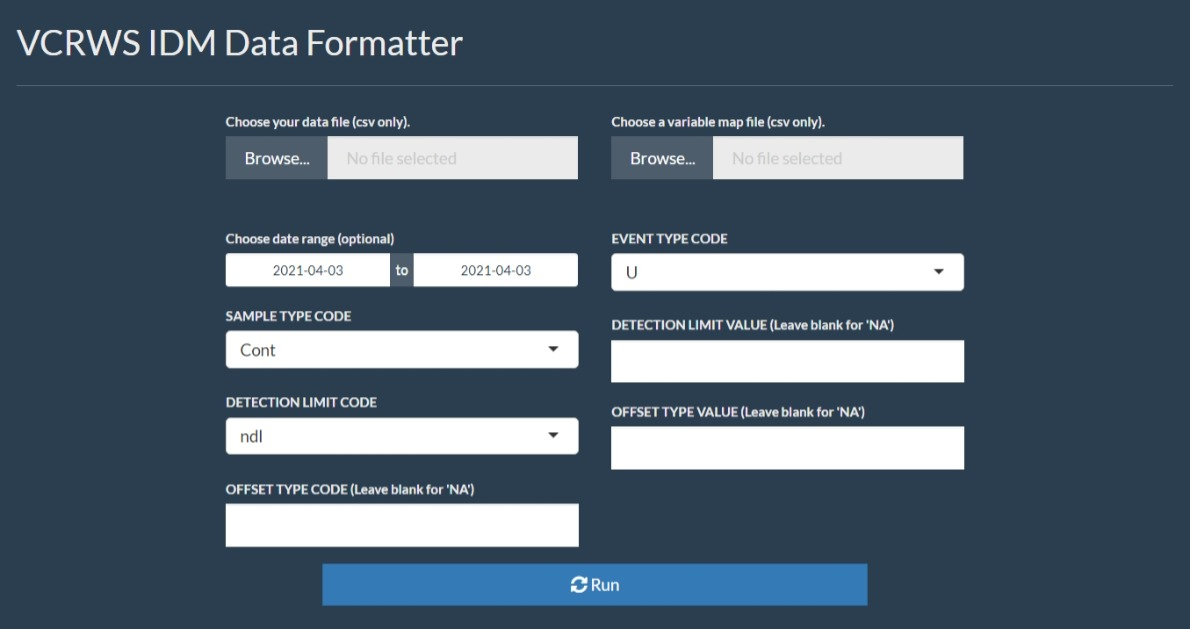
\includegraphics[width=0.8\textwidth]{gfx/chapter-storage/data-formatter.jpeg}
	\caption[R Shiny web app for data formatting.]{R Shiny web app for data formatting (Smith et al., submitted).}
	\label{fig:data-formatter}
\end{figure}




\subsection{Query Performance}

The SIDM web application consists of several pages for uploading data, managing user authentication and authorization, and creating new controlled language for expanding the available metadata.
User accessible pages include a map of all sites showing relative locations with links to a brief site description (Figure \ref{fig:idm-homepage}).

\begin{figure}[ht]
	\centering
	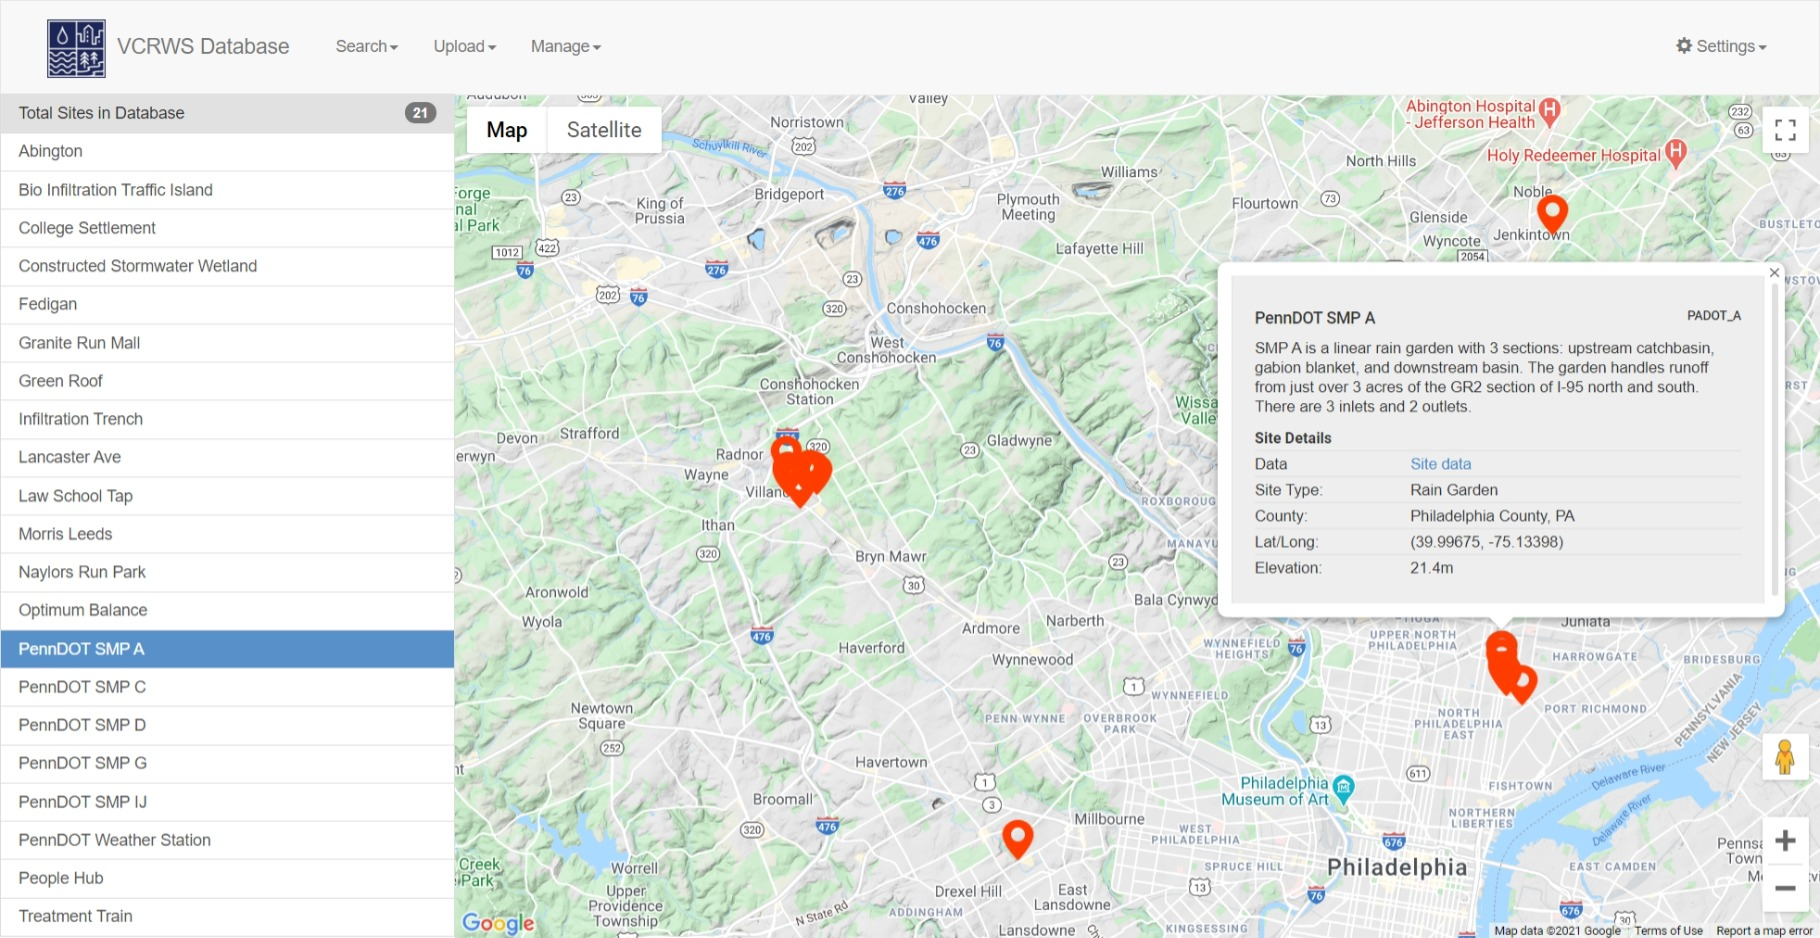
\includegraphics[width=0.8\textwidth]{gfx/chapter-storage/idm-homepage.jpeg}
	\caption{SIDM homepage showing geographical details for SMP A.}
	\label{fig:idm-homepage}
\end{figure}

The query builder page has filter selectors for each metadata parameter that allow a user to select one or more data identifiers, as well as a date range filter.
Once run, the query returns a paginated table of all data requested and gives the option to plot the points in single or multi-axis plots or to download the raw values for analysis in another software package.
The query page is also available to outside users who have access through data sharing links so that project partners can easily access the data.

Query performance is fairly quick given the size of data stored in the SIDM (100M+ data values recorded across all sites as of writing).
Current performance is reflected in \ref{table:query-performance}, and shows a sampling of common queries.
The indexing operations required for this improved performance mean that importing data takes longer than it otherwise would without the need to create indices.
This tradeoff is appropriate because many more query operations than import operations are expected, so the overall computational time is decreased, and compute time is more expensive than the increase in storage space consumed by indices.

\begin{table}[ht!]
\centering
\caption[SIDM query performance benchmarks.]{SIDM query performance benchmarks (Smith et al., submitted).}
	\begin{tabular}{| c | c | c | c | c |}
		\hline
		\multirow{2}{*}{Benchmark} & \multirow{2}{*}{Specifications} & \multicolumn{3}{c}{Performance (seconds to completion)} \vline \\ \cline{3-5}
		& & Query & Export to File & Graph + Statistics \\ \hline
		Small Dataset & \makecell{5 Sample Locations, \\ 6 Variables, \\ 900 Data Points, \\ 57.1KB } & 0.062 & 8.27  & 1.11 \\ \hline
		Large Dataset & \makecell{2 Sample Locations, \\ 2 Variables, \\ 955,762 Data Points, \\ 65.5MB } & 3.62 & 30.51 & 7.73 \\ \hline
	\end{tabular}
	\label{table:query-performance}
\end{table}

\section{Future Work}

\subsection{Streaming Data Ingest}
Currently, the process of extracting, transforming, and loading (ETL) data from the data loggers into the SIDM requires manual input and transfer of files.
Currently, each data logger appends data to a separate file on a remote server, which is accessed monthly to check the data, transform it, and load it into the SIDM.
The process is time consuming, subject to human error, and means that delays of data reaching the SIDM of a month or more are typical.
A better approach would be automatic streaming and loading of the data logger output directly to the SIDM on a close to real-time basis.
An update to the Campbell Scientific CR6 data logger's operating system, which is commonly used in VCRWS monitoring programs, enables the use of the message queueing telemetry transport (MQTT) framework.
MQTT is an internet-of-things (IoT) system that provides a lightweight method for sending and receiving data measurements between smart devices and servers (\cite{MQTT}).
An update to the SIDM could include an API to which the CR6 data loggers can send MQTT messages with up-to-date measurements, greatly enhancing the ability of the platform to automatically ingest new data.
A set of rules for each site and each variable could be used to further enhance this process by evaluating each incoming data point against a set of pre-specified criteria to ensure the integrity of the data or send alerts to users if measurements are out of bounds.
This ingestion system will have the added benefit of requiring more strict linking of physical sensors with their data stores and the rules used to define valid data immediately upon deployment.
Similar data loggers that already have remote connection capabilities could easily have data streaming capabilities enabled via a firmware update.

\subsection{Programmatic Data Retrieval}
The data sharing system of the ODM was removed from the SIDM's feature set to limit the publicity of preliminary data and protect research sponsors who wish to keep their data private.
While there are new methods for sharing specific query results, these still revolve around downloading CSV files containing the data.
There are no methods for programmatically sharing data or querying the database.
Analysis relies on correctly identifying and downloading data prior to beginning analysis, making individual queries difficult to communicate to other researchers.

Modern API design should be used to extend the existing query builder to allow any programming language access to the results of a query through javascript object notation (JSON), a common method for sending large data payloads using the HTTP protocol.
Every common programming language (R, python, MATLAB) used in statistical and modeling efforts supports making HTTP requests and handling JSON response data.
An analysis script could query this API endpoint with the requirements for a dataset of interest and store the server's response before continuing with the necessary calculations.
This would reduce the amount of time required for analysis as a user can directly load data from the server into their analysis program of choice without the need to shuffle data files around, and gathering new data becomes as simple as resending the query request to the server.

\section{Conclusions}

Making data storage FAIR means that data is easily accessible, and analyses performed within a site become easier to transfer to similar sites.
The ability to scale analysis across multiple sites will greatly expand the scope of research that is able to be conducted on larger GSI systems.
This is accomplished through controlled vocabulary for describing data and consistent, yet flexible, formatting of the database schema.
Allowing the addition of new variables at any site or sampling location means that the database can continue to be expanded with new sites and variables without losing the integrity of the historical data already captured.
Furthermore, the increasing accessibility of continuous monitoring through inexpensive IoT devices will mean that future sites are able to be monitored and added to the database easily, greatly expanding the value of consistent formatting and data descriptions.
More specifically, it will be possible to understand how individual systems' performance impacts a larger system.
Finally, VCRWS' SIDM has made significant progress in accomplishing these goals, as VCRWS data stretching back to 2003 across many sites is now contained in a single format.
The SIDM will unlock the potential for expanded collaboration between researchers, better understandings of long-term monitoring results, and more robust analyses of multi-site GSI systems.
